% use `pdflatex -shell-escape Perfect_Circumplex.tex` in the terminal

\documentclass[border={10pt 10pt 10pt 10pt},crop,tikz,convert={outext=.svg,command=\unexpanded{pdf2svg \infile\space\outfile}},multi=false]{standalone}
\usepackage[utf8]{inputenc}
\usepackage{todonotes}
\usetikzlibrary{decorations.pathmorphing, decorations.text}



\usepackage{babel}[ngerman]
%\usepackage{fontspec}
%\setmainfont{Arial}
\tikzstyle{every picture}+=[font=\sffamily]


\begin{document}
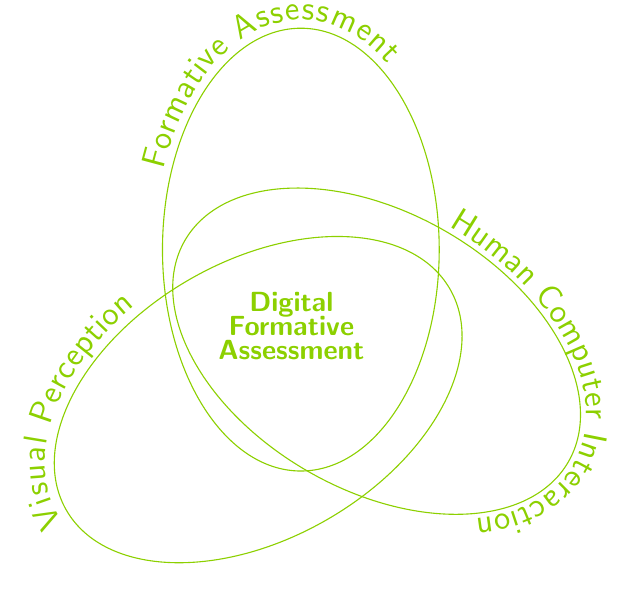
\begin{tikzpicture}
\definecolor{phgreen}{RGB}{140,208,0} 
%%     
\draw[color=phgreen, rotate= 60,
 postaction={decorate,
    decoration={raise=.2em, 
    text along path, pre length=0cm, reverse path,
      text={|\color{phgreen}\sffamily \large|Human Computer Interaction},
    }}] (2,-3) arc (0:360:50pt and 80pt);  
  
%\setsansfont[Ligatures=TeX]{Arial}
%%     
\draw[color=phgreen, rotate=120, 
 postaction={decorate,
    decoration={raise=.35em, 
    text along path, pre length=10.8cm, reverse path,
      text={| \color{phgreen}\sffamily \large|Visual Perception},
    },
  }] (-.5,-.1) arc (0:360:50pt and 80pt);
  


%%     
\draw[color=phgreen, rotate=180, 
 postaction={decorate,
    decoration={raise=0.3em, 
    text along path, pre length=1cm, reverse path,
      text={|\color{phgreen}\sffamily \large|Formative Assessment},
    },
  }] (0,0) arc (0:360:50pt and 80pt);
  



%% Labels
\draw (1.5,-1) node [text=phgreen, text width=2cm]{  
  \tiny
  \begin{tabular}{c}
    \normalsize \textbf{Digital}\\ \normalsize \textbf{Formative}\\ \normalsize \textbf{Assessment}
  \end{tabular}};
  

 
 
 
\end{tikzpicture}
\end{document}
